\section{RQ4: Model-level decisions under a fixed pipeline}
\label{sec:model}

\subsection{Compression screening and a resolution router: negative results}
\label{sec:compression}

Before the pipeline study, we spent most of our effort on the model:
L1 and gradient-based channel pruning, mixed-precision QAT,
distillation, and a per-image router that chooses between a 512 and a
640 engine from pre-inference statistics. Under a common short
recovery budget (1,024 development images, five epochs, one seed) none
of the compressed variants reduced compiled engine time at acceptable
accuracy, and the router, which looked favorable on its fitting split,
lost AP and small-object recall on an independent hash-verified
verification split, so we rejected it. \Cref{app:compression} reports
both campaigns in full. These results do not show that compression
cannot work. They show something narrower: for a 2.6\,M-parameter
NMS-free detector on this device and budget, the achievable
engine-time savings are a small fraction of the 3$\times$ governor
effect of \cref{sec:diagnosis} --- which is why the rest of this
section varies resolution and model size while holding the
optimization budget fixed.

\subsection{The value of a lower input resolution depends on the schedule}
\label{sec:resolution}

Lowering the input resolution is the cheapest model-level saving
available. It needs no training, only a new engine. \Cref{fig:resolution}
compares static 512, 576 and 640 engines of the same pretrained YOLO26n
checkpoint on all of val2017, in the naive pipeline (float input,
sequential, stream sync) and in the full pipeline. Accuracy falls from
0.4026 AP (640) to 0.3864 (576) and 0.3748 (512). AP$_S$ falls from 0.198
to 0.175 and 0.160. In the naive pipeline, 512 buys 27\% more throughput
(34.3 to 43.4 images/s) and 22\% less energy per image. In the full
pipeline the same saving shrinks to a few percent: 214.6, 222.2 and
218.7 images/s for 640, 576 and 512 ($+3.5$\% and $+1.9$\%; the
repeat ranges of the lower resolutions lie above the 640 range, so
the gain is small but consistent across the two repeats). The pipeline is now limited by the main thread
(\cref{sec:ladder}): at 1020\,MHz the engine's 4.2\,ms sits just below
the ${\approx}4.7$\,ms per-image period the host stages impose, so most
of the engine time saved by a smaller input is absorbed by the
unchanged per-image host work.

Part of that saturation is Python. Re-running the same comparison with
CPython's cyclic garbage collector disabled (\texttt{gc.disable()},
identical predictions) raises all three throughputs to 229.9, 244.0 and
252.1 images/s, and the resolution spread widens to $+6.1$\% (576) and
$+9.7$\% (512). Cyclic-GC pauses on the main thread absorb a further
share of the saved engine time; with them removed, a lower input
resolution still buys roughly a third of what it buys in the naive
pipeline, not a negligible amount. The host work that remains ---
the main thread's per-image period
(\cref{sec:ladder}) --- depends on the source image and the pipeline,
not on the network input. The energy benefit is robust either way:
73.7 to 58.0\,mJ per image (21\%) on a backlog with the default
collector, and 71.2 to 55.8\,mJ (22\%) with it disabled, because the
GPU finishes each inference sooner. The same 2.8 AP
points therefore buy a large throughput gain in a naive pipeline and a
much smaller one in an optimized pipeline --- $2$--$10$\% depending on
host-runtime hygiene. A compression or resolution decision evaluated in a naive
pipeline, or in \texttt{trtexec}, does not carry over to an optimized one.

\begin{figure}[t]
\centering
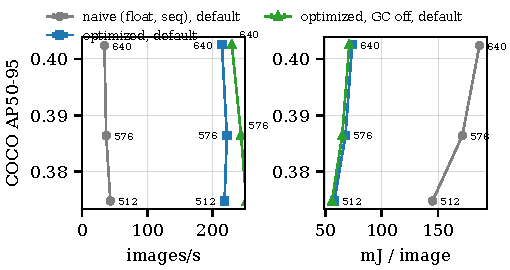
\includegraphics[width=\columnwidth]{figs/resolution.pdf}
\caption{COCO val2017 AP against throughput (images/s) and energy per
image (mJ) for
static 512/576/640 YOLO26n engines, default governors, mean of two runs
(whiskers: repeat min/max; labels: input size).
In the full pipeline (squares), lower resolution buys only $2$--$4$\%
throughput because the pipeline is limited by the main thread, not by
GPU throughput (the GPU already runs at its maximum clock); disabling
CPython's cyclic GC (triangles, identical predictions) raises all three
points and widens the spread to $6$--$10$\%.}
\label{fig:resolution}
\end{figure}


\subsection{Generality: YOLO26s and YOLOv10n}
\label{sec:generality}

\begin{table*}[t]
\centering
\caption{Other NMS-free detectors on all 5,000 val2017 images, 640, batch 1
(default: mean of two runs; locked: one run). ``Naive'' is float input with sequential execution and
stream synchronization; ``full'' is uint8 input, two prefetch workers, overlap
and event synchronization. MHz is the mean sampled GPU clock under the
default governor.}
\label{tab:generality}
\small
\setlength{\tabcolsep}{2.6pt}
\begin{tabular}{llcc rrrr rr}
\toprule
& & & & \multicolumn{4}{c}{Default} & \multicolumn{2}{c}{Locked} \\
\cmidrule(lr){5-8} \cmidrule(lr){9-10}
Model & Pipeline & AP & AP$_S$ & img/s & mJ & W & MHz & img/s & mJ \\
\midrule
YOLO26s & Ultralytics & 0.4769 & 0.3020 & 25.1 & 263.5 & 6.62 & 306 & 63.0 & 194.4 \\
 & Ours, naive & 0.4770 & 0.3019 & 24.5 & 271.6 & 6.66 & 306 & 52.2 & 221.8 \\
 & Ours, full & 0.4769 & 0.3019 & 140.1 & 131.8 & 18.47 & 1019 & 140.4 & 133.3 \\ \midrule
YOLOv10n & Ultralytics & 0.3836 & 0.1901 & 30.8 & 198.4 & 6.12 & 306 & 73.0 & 144.5 \\
 & Ours, naive & 0.3837 & 0.1900 & 33.5 & 189.4 & 6.34 & 306 & 60.0 & 167.4 \\
 & Ours, full & 0.3839 & 0.1901 & 212.4 & 76.9 & 16.33 & 1018 & 215.2 & 77.8 \\
\bottomrule
\end{tabular}
\end{table*}


\Cref{tab:generality} repeats the three main configurations for
YOLO26s (10.0\,M parameters) and YOLOv10n. In every case the three
pipelines agree in AP to within $4\times10^{-4}$, and the naive
pipelines run the GPU at 306\,MHz under default governors. YOLOv10n
behaves like YOLO26n: 30.8 images/s with Ultralytics and 212.4 with the
full pipeline ($6.9\times$), at 76.9 instead of 198.4\,mJ per image.
YOLO26s has $3.9\times$ the parameters of YOLO26n and a $1.6\times$
longer engine time (6.78 versus 4.22\,ms back-to-back). Its full
pipeline is limited by the GPU rather than the CPU. It reaches
140.1 images/s ($5.6\times$ Ultralytics), 95\% of the 146.9
inferences/s that \texttt{trtexec} achieves back-to-back, and locking
clocks does not change it (140.4). Under the default governors, the full
YOLO26s pipeline outruns the Ultralytics YOLO26n predictor with locked
clocks (140.1 vs.\ 73.9 images/s) at 0.074 higher AP and 7.5\,mJ less
per image (131.8 vs.\ 139.3). This comparison changes the pipeline and
the model at once, so it does not show that the larger model is the
better choice; YOLO26n in the same full pipeline is faster still. It
shows that the larger model costs less than a naive pipeline, even one
running with locked clocks. A deployment decision that compares model
sizes in a naive pipeline therefore mostly measures the pipeline.


\textbf{Answer to RQ4.}
Once the pipeline is fixed, model-level savings matter much less than
the engine benchmark suggests. A 2.8-point AP sacrifice for a lower
resolution yields 27\% more throughput in a naive pipeline but only
2--4\% in an optimized one (6--10\% with cyclic GC disabled), plus lower
energy on a backlog. Our
compression variants did not reduce compiled engine time at
acceptable accuracy within the budget screened.
The router saved at most one eleventh of what scheduling saved, and it failed held-out verification. Whether the schedule effects carry over to other detectors and other accelerators is \RQ{5} (\cref{sec:crossplatform}); within this section, YOLOv10n and YOLO26s show speedups of $5.6$--$6.9\times$ over the Ultralytics predictor, and for YOLO26s, whose engine is $1.6\times$ slower than YOLO26n's, the pipeline effect is large enough that the choice of pipeline matters more for throughput than the choice between the two model sizes.

